\documentclass{article}
\usepackage[UKenglish]{babel}
\usepackage[UKenglish]{isodate}
\usepackage{fullpage}
\usepackage{amsmath,amssymb,amsthm}
\usepackage{bm}
\usepackage{bbm}
\usepackage{mathtools}
\usepackage{url}
\usepackage{graphicx}

\newtheorem{theorem}{Theorem}[section]
\newtheorem{proposition}[theorem]{Proposition}
\newtheorem{lemma}[theorem]{Lemma}
\newenvironment{proofsketch}{%
  \renewcommand{\proofname}{Proof sketch}\proof}{\endproof}
\theoremstyle{definition}
\newtheorem{definition}[theorem]{Definition}
\theoremstyle{remark}
\newtheorem*{remark}{Remark}

\DeclareMathOperator{\tr}{tr}
\DeclareMathOperator{\diag}{diag}
\DeclareMathOperator{\adj}{adj}

\newcommand{\Eq}{\mathbb{E}_{(\mathbf{u}, \mathbf{r}) \sim \approximation}}
\newcommand{\pfull}{p(\mathcal{D}, \mathbf{u}, \mathbf{r})}
\newcommand{\approximation}{q_{\bm\nu}(\mathbf{u}, \mathbf{r})}
\newcommand{\Kuu}{\mathbf{K}_{\mathbf{u},\mathbf{u}}}
\newcommand{\Luu}{\mathbf{L}_{\mathbf{u},\mathbf{u}}}
\newcommand{\Krr}{\mathbf{K}_{\mathbf{r},\mathbf{r}}}
\newcommand{\Kru}{\mathbf{K}_{\mathbf{r},\mathbf{u}}}
\newcommand{\V}{V_{\mathbf{r}}}

\newcommand{\dm}{\frac{\partial}{\partial\bm\mu}}
\newcommand{\dS}{\frac{\partial}{\partial\mathbf{S}}}
\newcommand{\dD}{\frac{\partial}{\partial\mathbf{D}}}
\newcommand{\dB}{\frac{\partial}{\partial\mathbf{B}}}
\newcommand{\dt}{\frac{\partial}{\partial t}}
\newcommand{\dl}{\frac{\partial}{\partial \lambda_i}}
\newcommand{\dlj}{\frac{\partial}{\partial \lambda_j}}

\newcommand{\f}{f(\mathbf{r}, \mathbf{u}, t)}
\newcommand{\ftn}{f(\mathbf{r}, \mathbf{u}, t_n)}
\newcommand{\fn}{f_n(\mathbf{r}, \mathbf{u})}
\newcommand{\dx}{\,d\mathbf{r}\,d\mathbf{u}}
\newcommand{\df}{\left.\frac{\partial f}{\partial t}\right|_{(\mathbf{r},
    \mathbf{u}, t)}}
\newcommand{\g}{g(\mathbf{r}, \mathbf{u})}
\newcommand{\rinf}{\lVert \mathbf{r} \rVert_\infty}
\newcommand{\vbound}{\frac{\rinf + \log|\mathcal{A}|}{1 - \gamma}}

\DeclarePairedDelimiterX{\infdivx}[2]{(}{)}{%
  #1\;\delimsize\|\;#2%
}
\newcommand{\DKL}{D_{\mathrm{KL}}\infdivx}

\title{Variational Inference for Inverse Reinforcement Learning with Gaussian
  Processes: Supplementary Material}
\author{Paulius Dilkas (2146879)}

\begin{document}
\maketitle

\begin{proof}
  \leavevmode
  \begin{enumerate}
  \item
    \[
      \begin{split}
        \frac{\partial q(\mathbf{u})}{\partial m} &=
        q(\mathbf{u})\dm\left[-\frac{1}{2}(\mathbf{u} -
          \bm\mu)^\intercal\bm\Sigma^{-1}(\mathbf{u} - \bm\mu)\right]
        \\
        &= -\frac{1}{2}q(\mathbf{u})(\bm\Sigma^{-1} +
        \bm\Sigma^{-\intercal})(\mathbf{u} - \bm\mu)\dm[\mathbf{u} -
        \bm\mu] \\
        &= \frac{1}{2}q(\mathbf{u})(\bm\Sigma^{-1} +
        \bm\Sigma^{-\intercal})(\mathbf{u} - \bm\mu).
      \end{split}
    \]
  \item For $\mathbf{S} \in \{ \bm\Sigma, \mathbf{B}, \mathbf{D} \}$,
    \begin{align}
      \frac{\partial q(\mathbf{u})}{\partial \mathbf{S}} &= \dS\left[\frac{1}{(2\pi)^{m/2}|\bm\Sigma|^{1/2}}\exp \left( -\frac{1}{2} (\mathbf{u} - \bm\mu)^\intercal\bm\Sigma^{-1}(\mathbf{u} - \bm\mu)\right)\right] \nonumber \\
                                                         &= \dS\left[\frac{1}{(2\pi)^{m/2}|\bm\Sigma|^{1/2}}\right]\exp \left( -\frac{1}{2} (\mathbf{u} - \bm\mu)^\intercal\bm\Sigma^{-1}(\mathbf{u} - \bm\mu)\right) \nonumber \\
                                                         &+ \frac{1}{(2\pi)^{m/2}|\bm\Sigma|^{1/2}}\dS\left[\exp\left( -\frac{1}{2} (\mathbf{u} - \bm\mu)^\intercal\bm\Sigma^{-1}(\mathbf{u} - \bm\mu)\right)\right] \nonumber \\
                                                         &= -\frac{1}{2} q(\mathbf{u}) \left( |\bm\Sigma|^{-3/2} \frac{\partial |\bm\Sigma|}{\partial \mathbf{S}} + \dS[(\mathbf{u} - \bm\mu)^\intercal\bm\Sigma^{-1}(\mathbf{u} - \bm\mu)] \right). \label{eq:2_before}
    \end{align}
    For derivatives with respect to $\bm\Sigma$, we can refer to Petersen and
    Pedersen \cite{petersen2008matrix}:
    \begin{equation} \label{eq:partial_derivatives1}
      \begin{gathered}
        \frac{\partial |\bm\Sigma|}{\partial \bm\Sigma} =
        |\bm\Sigma|\bm\Sigma^{-\intercal}, \\
        \dS[(\mathbf{u} - \bm\mu)^\intercal\bm\Sigma^{-1}(\mathbf{u} -
        \bm\mu)] = -\bm\Sigma^{-\intercal}\mathbf{U}\bm\Sigma^{-\intercal},
      \end{gathered}
    \end{equation}
    while we can use an online tool by Laue et
    al.\footnote{\url{http://www.matrixcalculus.org/}}
    \cite{DBLP:conf/nips/LaueMG18} for the remaining ones:
    \begin{equation} \label{eq:partial_derivatives2}
      \begin{gathered}
        \frac{\partial |\bm\Sigma|}{\partial \mathbf{B}} =
        (\adj(\mathbf{T}) + \adj(\bm\Sigma))\mathbf{B}, \\
        \frac{\partial |\bm\Sigma|}{\partial \mathbf{D}} =
        \adj(\mathbf{T})\mathbf{D}^\intercal + \mathbf{D}^\intercal
        \adj(\mathbf{T}), \\
        \dB[(\mathbf{u} - \bm\mu)^\intercal\bm\Sigma^{-1}(\mathbf{u} -
        \bm\mu)] = -(\mathbf{TUT} +
        \bm\Sigma^{-1}\mathbf{U}\bm\Sigma^{-1})\mathbf{B}, \\
        \dD[(\mathbf{u} - \bm\mu)^\intercal\bm\Sigma^{-1}(\mathbf{u} - \bm\mu)] =
        -\mathbf{T}\mathbf{UT}\mathbf{D}^\intercal -
        \mathbf{D}^\intercal\mathbf{T}\mathbf{UT}.
      \end{gathered}
    \end{equation}
    Substituting results from \eqref{eq:partial_derivatives1} and
    \eqref{eq:partial_derivatives2} back into \eqref{eq:2_before} gives:
    \begin{gather*}
      \frac{\partial q(\mathbf{u})}{\partial \bm\Sigma} =
      \frac{1}{2}q(\mathbf{u})(\bm\Sigma^{-\intercal}\mathbf{U}\bm\Sigma^{-\intercal}
      - \bm\Sigma^{-\intercal}), \\
      \frac{\partial q(\mathbf{u})}{\partial \mathbf{B}} =
      \frac{1}{2}q(\mathbf{u}) \{ |\bm\Sigma|^{-3/2}(\adj(\mathbf{T}) +
      \adj(\bm\Sigma)) + \mathbf{TUT} +
      \bm\Sigma^{-1}\mathbf{U}\bm\Sigma^{-1} \} \mathbf{B}, \\
      \frac{\partial q(\mathbf{u})}{\partial \mathbf{D}} =
      \frac{1}{2}q(\mathbf{u}) \{ \mathbf{T}\mathbf{UT}\mathbf{D}^\intercal +
      \mathbf{D}^\intercal\mathbf{T}\mathbf{UT} -
      |\bm\Sigma|^{-3/2}(\adj(\mathbf{T})\mathbf{D}^\intercal +
      \mathbf{D}^\intercal \adj(\mathbf{T})) \}.
    \end{gather*}
  \item Using a result by Rasmussen and Williams % TODO: update the proof
                                % according to the new result
    \cite{DBLP:books/lib/RasmussenW06},
    \[
      \frac{\partial q(\mathbf{r} \mid \mathbf{u})}{\partial \lambda_i} =
      q(\mathbf{r} \mid \mathbf{u}) \dl
      \left[-\frac{1}{2}\mathbf{u}^\intercal\Kuu^{-1}\mathbf{u} -
        \frac{1}{2}\log|\Kuu| \right] = \frac{1}{2}q(\mathbf{r} \mid \mathbf{u})\tr
      \left((\Kuu^{-1}\mathbf{u}\mathbf{u}^\intercal\Kuu^{-\intercal} -
        \Kuu^{-1}) \frac{\partial \Kuu}{\partial \lambda_i} \right).
    \]
    The remaining derivative is
    \[
      \frac{\partial \Kuu}{\partial \lambda_i} =
      \begin{cases}
        \frac{1}{\lambda_i}\Kuu & \text{if } i = 0, \\
        \Luu & \text{otherwise,}
      \end{cases}
    \]
    where
    \[
      \begin{split}
        [\Luu]_{j,k} &= \dl k_{\bm\lambda}(\mathbf{x}_{\mathbf{u},j},
        \mathbf{x}_{\mathbf{u},k}) \\
        &= k_{\bm\lambda}(\mathbf{x}_{\mathbf{u},j}, \mathbf{x}_{\mathbf{u},k})
        \dl \left[-\frac{1}{2}(\mathbf{x}_{\mathbf{u},j} -
          \mathbf{x}_{\mathbf{u},k})^\intercal \bm\Lambda
          (\mathbf{x}_{\mathbf{u},j} - \mathbf{x}_{\mathbf{u},k}) -
          \mathbbm{1}[j \ne k]\sigma^2\tr(\bm\Lambda) \right] \\
        &= k_{\bm\lambda}(\mathbf{x}_{\mathbf{u},j}, \mathbf{x}_{\mathbf{u},k})
        \dl \left[-\frac{1}{2}\sum_{l=1}^d \lambda_l
          (x_{\mathbf{u},j,l} - x_{\mathbf{u},k,l})^2 -
          \mathbbm{1}[j \ne k]\sigma^2\sum_{l=1}^d \lambda_l \right] \\
        &= k_{\bm\lambda}(\mathbf{x}_{\mathbf{u},j}, \mathbf{x}_{\mathbf{u},k})
        \left( -\frac{1}{2}(x_{\mathbf{u},j,i} -
        x_{\mathbf{u},k,i})^2 - \mathbbm{1}[j \ne k]\sigma^2 \right).
      \end{split}
    \]
  \end{enumerate}
\end{proof}

\begin{figure}
  \centering
  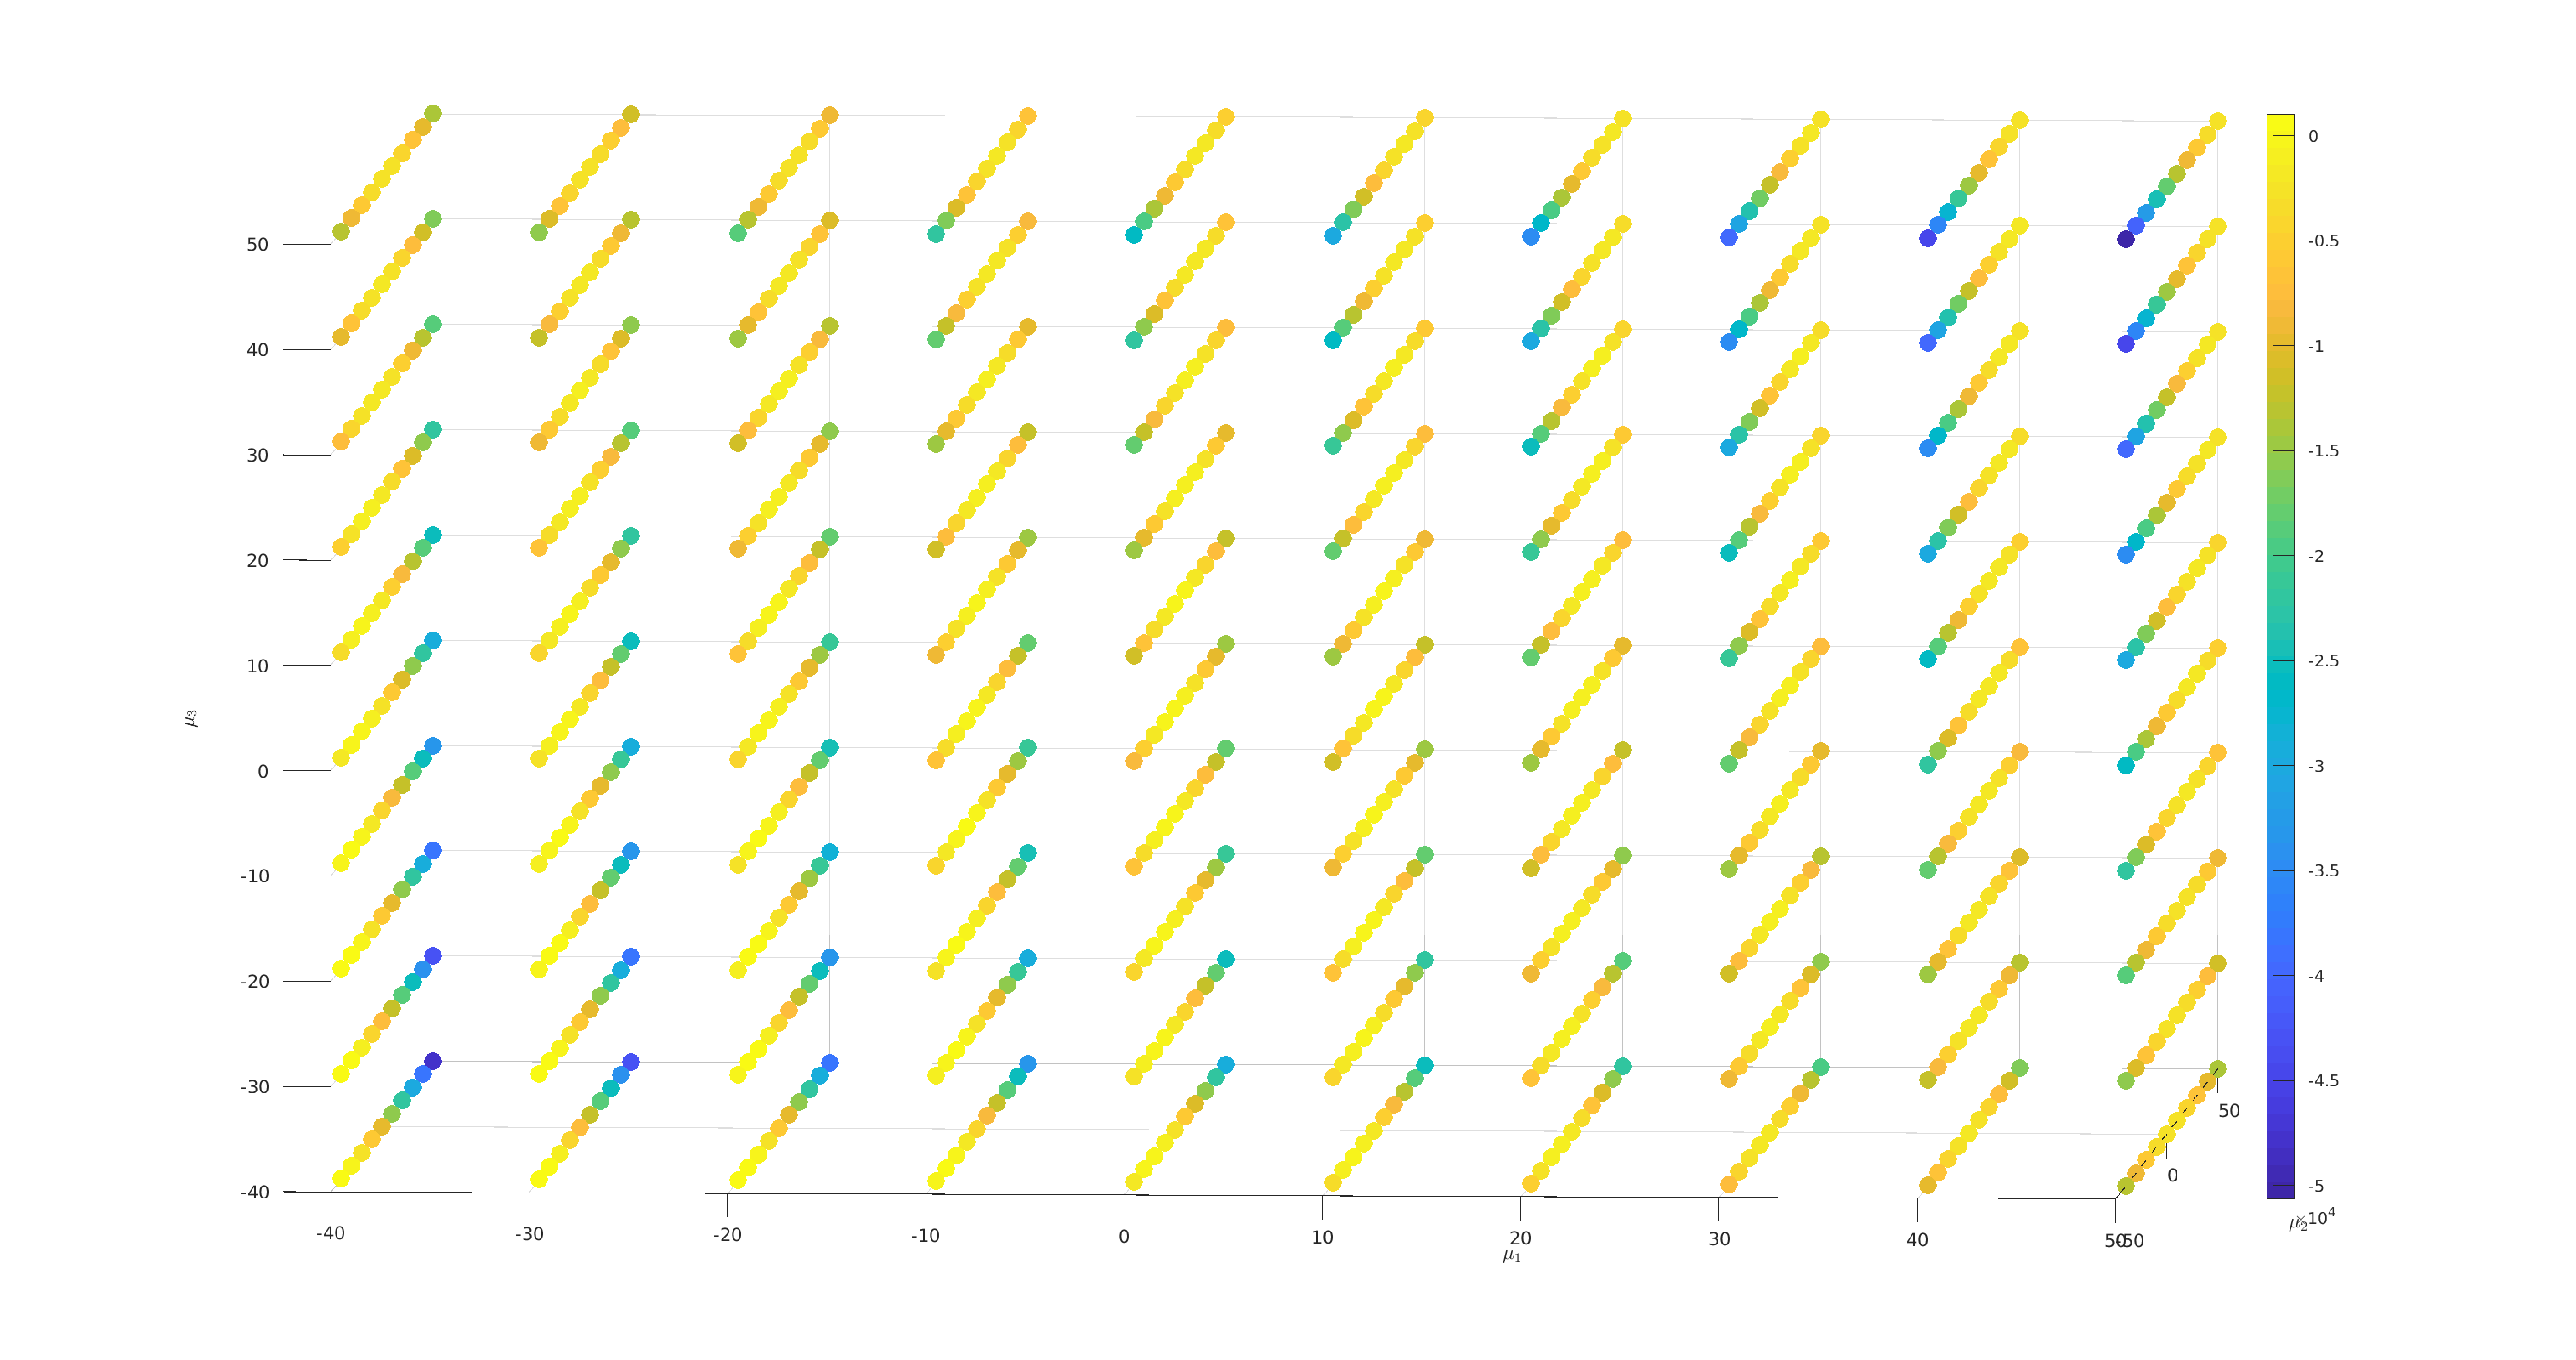
\includegraphics[width=\textwidth]{elbo_over_mu}
\end{figure}

\bibliographystyle{abbrv}
\bibliography{paper.bib}
\end{document}